\documentclass[11pt]{article}

\usepackage{amsmath}
\usepackage{graphicx}
\usepackage{float}
\usepackage{upgreek}

\title{1. Ohmov zakon}
\author{Taj Šobot}

\begin{document}
    \maketitle
    \flushleft

    \section{1. zaporedna in vzporedna vezava}
    Fitan graf za enosmerni tok:
    \begin{figure}[H]
        \centering
        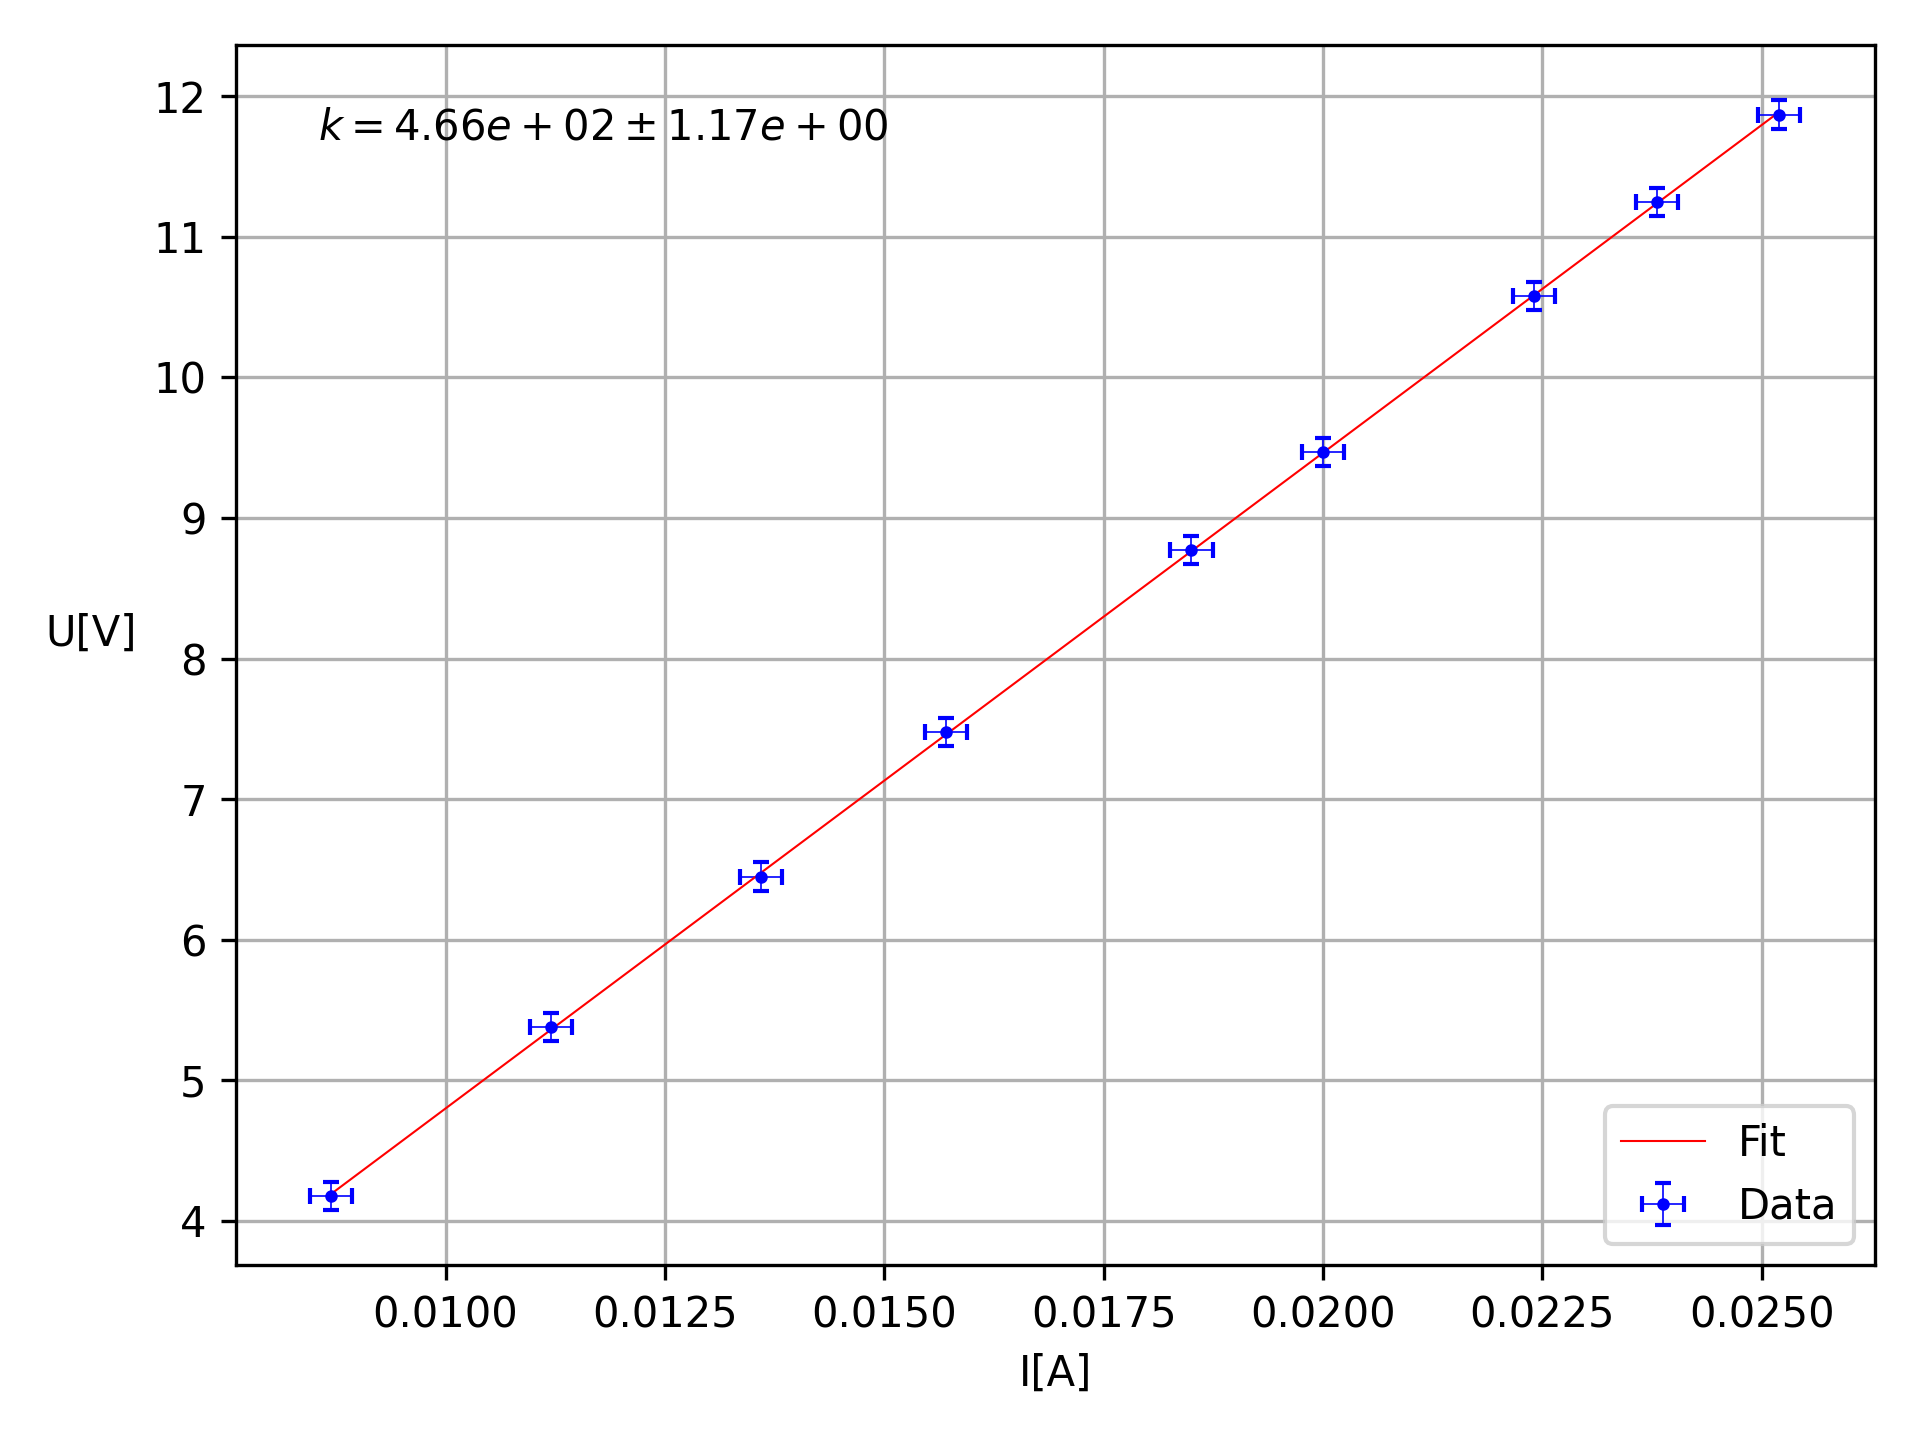
\includegraphics[width=0.9\textwidth]{graf1DC-}
        \caption{Graf1}
        \label{fig:1}
    \end{figure}

    \[
       R =(467 \pm 1)\Omega
    \]
    Fitan graf za izmenični tok:
    \begin{figure}[H]
        \centering
        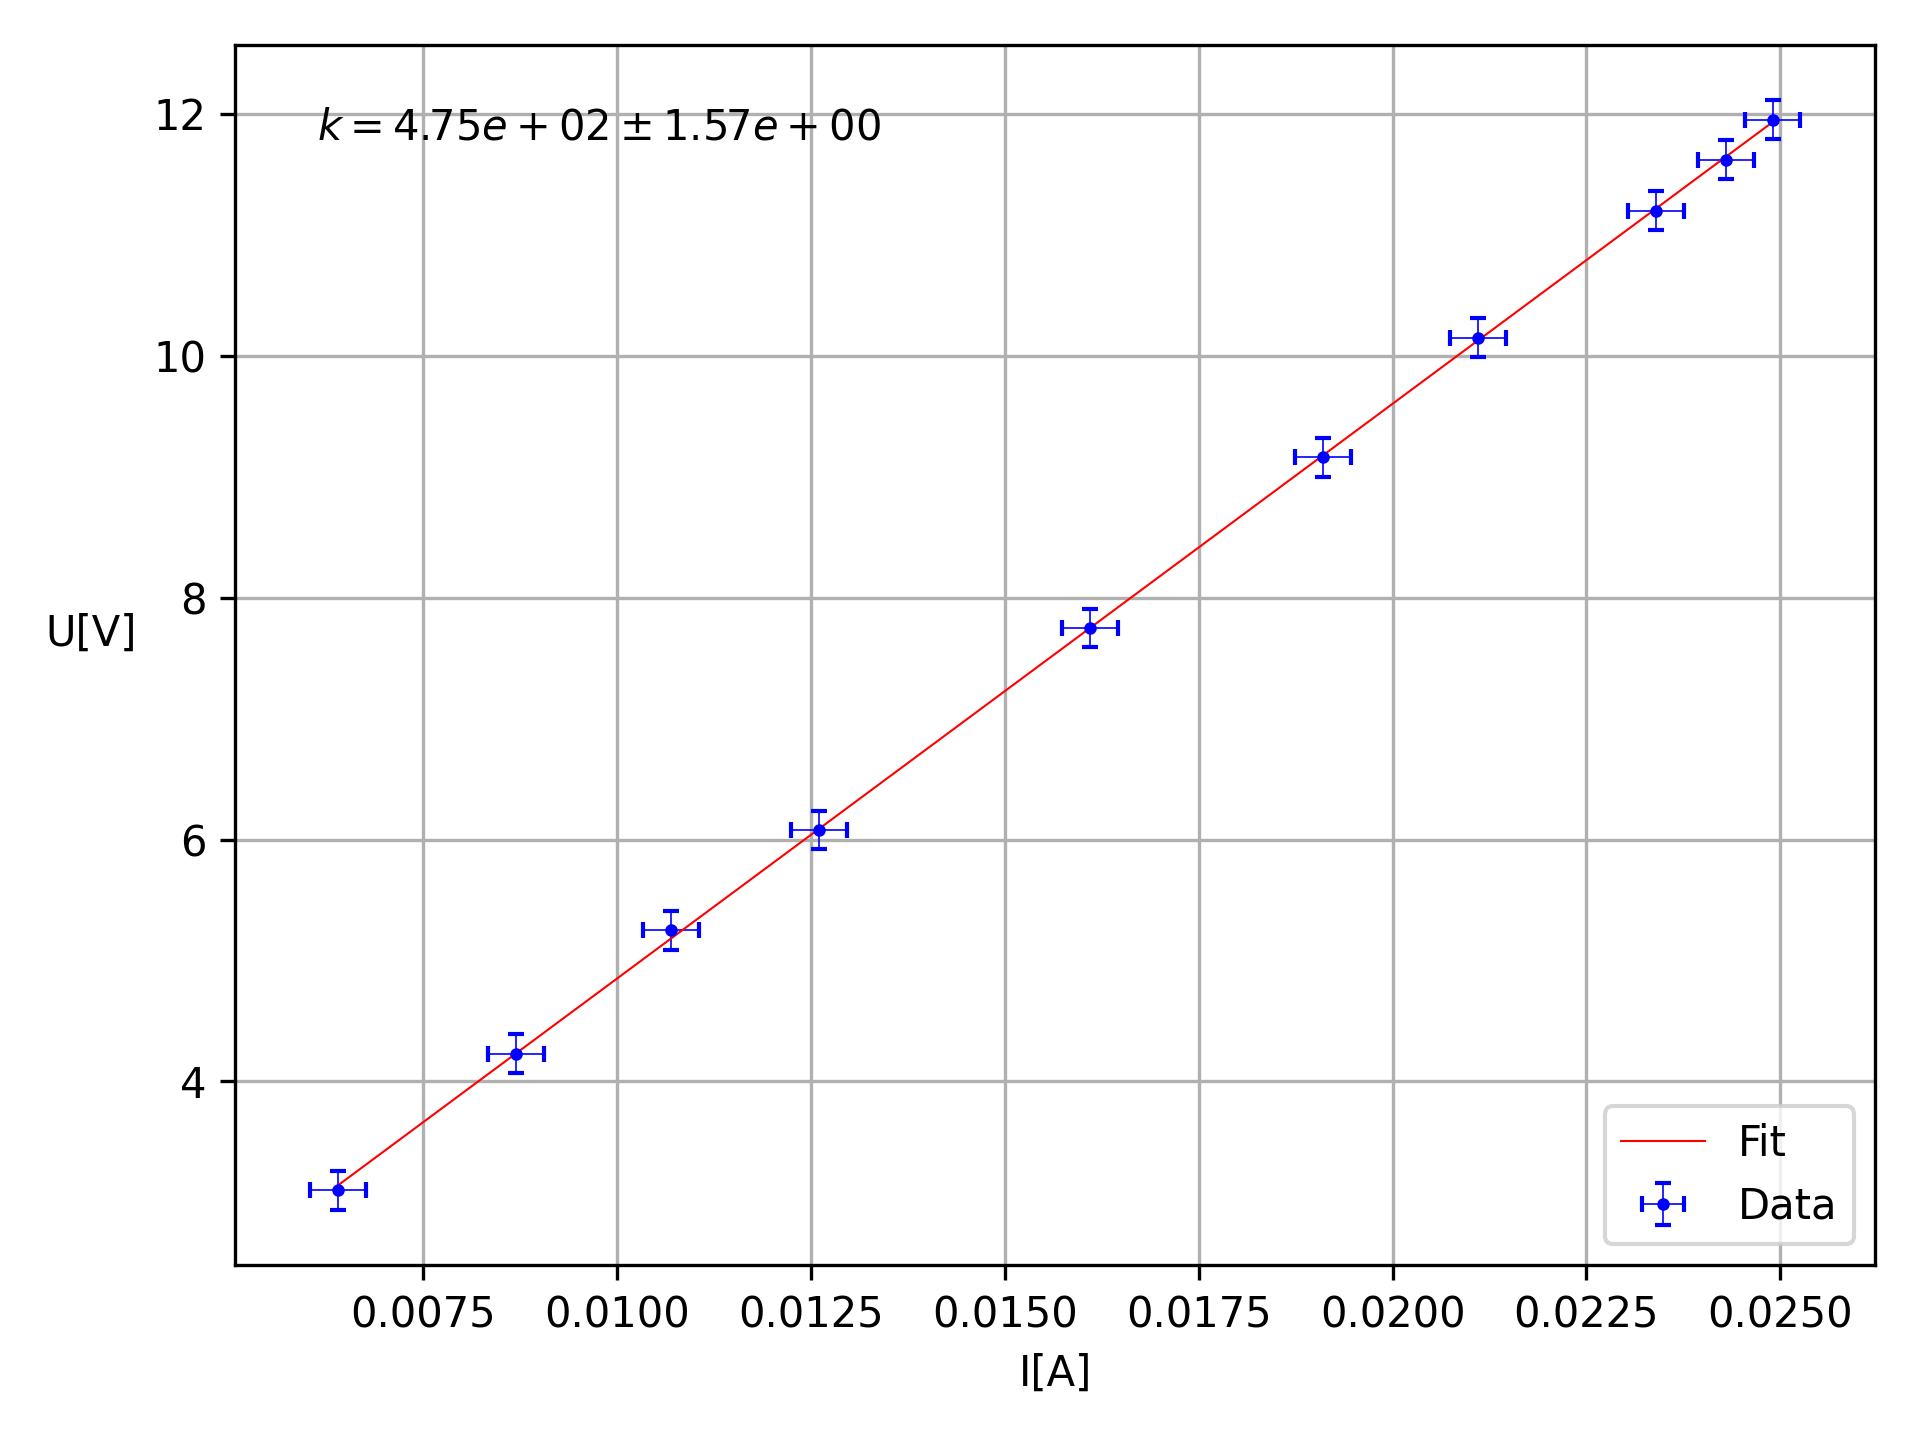
\includegraphics[width=0.9\textwidth]{graf1AC-}
        \caption{Graf2}
        \label{fig:2}
    \end{figure}

    \[
        R = (477 \pm 2) \Omega
    \]

    \section{2. velik upor}


\end{document}